\documentclass[handout, mathserif]{beamer}
\usepackage[nofirafonts]{beamerthemefocus}
\usepackage{amsmath}
\usepackage{graphicx}
\usepackage{xeCJK}
\usepackage{parskip}
\usepackage{xcolor}

\usepackage{listings}
\usepackage{xcolor}

\definecolor{codegreen}{rgb}{0,0.6,0}
\definecolor{codegray}{rgb}{0.5,0.5,0.5}
\definecolor{codepurple}{rgb}{0.58,0,0.82}
\definecolor{backcolour}{rgb}{0.95,0.95,0.92}

\lstdefinestyle{mystyle}{
    backgroundcolor=\color{backcolour},   
    commentstyle=\color{codegreen},
    keywordstyle=\color{magenta},
    numberstyle=\tiny\color{codegray},
    stringstyle=\color{codepurple},
    basicstyle=\ttfamily\footnotesize,
    breakatwhitespace=false,         
    breaklines=true,                 
    captionpos=b,                    
    keepspaces=true,                 
    % numbers=left,                    
    numbersep=5pt,                  
    showspaces=false,                
    showstringspaces=false,
    showtabs=false,                  
    tabsize=2
}

\lstset{style=mystyle}
\setCJKmainfont{Iansui 094 Regular}
\newcommand{\code}[1]{\texttt{#1}}
\newcommand{\given}{\mid}
\newcommand{\indep}{\perp \!\!\! \perp}

\title{CH7 習題演練}
\author{陳家威 \thanks{R10323045@ntu.edu.tw}}

\begin{document}
    \begin{frame}    
        \maketitle
    \end{frame}

    \section{7-9}
    \begin{frame}
    \frametitle{題幹}
    \begin{enumerate}
        \item 母親吸菸對出生嬰兒會不會有影響?
        \item 直覺會有影響,但是實證上能不能證明?
        \item 資料集為 bweight\_small
    \end{enumerate}
\end{frame}

\begin{frame}
    \frametitle{基本統計量}
    \begin{itemize}
        \item 母親吸菸者,出生嬰兒體重的平均值
        \item 母親不吸菸者,出生嬰兒體重的平均值
        \item 使用 t 檢定,檢定兩族群平均體重是否相同。
    \end{itemize}
\end{frame}

\begin{frame}
    \frametitle{分兩群做平均,能代表什麼嗎?}

    考慮以下問題:

    \begin{enumerate}
        \item 醫生平均年薪 300萬
        \item 高級社畜平均年薪 200萬
        \item 所以高級社畜去當醫生,年薪可以增加?
    \end{enumerate}
    \vfill
    請問哪裡怪怪的?

\end{frame}

\begin{frame}
    \frametitle{我們到底想量測什麼東西?}

    經濟學家有許多會想量測的「如果」問題,這些我們統稱為「處理效果」
    \begin{enumerate}
        \item[ATE] 如果隨機分配一個人去當醫生,他會比隨機分配他去當高級社畜多賺多少?
        \item[ATT] 如果醫生沒當醫生,那他少賺多少?
        \item[ATU] 如果把一個當了高級社畜的人抓去當醫生,他會多賺多少?
        \item[LATE] 對一個只差一點點就上醫學系的高級社畜,讓他真的當醫生,可以多賺多少?
    \end{enumerate}
    
    會需要考慮這麼多「處理效果」的原因,在於「結果通常不是隨機的」,而是「自我選擇的」
\end{frame}

\begin{frame}
    \frametitle{各種處理效果}
    \begin{table}
        \centering
        \begin{tabular}{c | l}
            \hline
            ATE & $E[Y_1] - E[Y_0]$ \\
            ATT & $E[Y_1 \mid D=1] - \begingroup \color{red} E[Y_0 \mid D=1]\endgroup$ \\
            ATU & $\begingroup \color{red}E[Y_1 \mid D=0] \endgroup -  E[Y_0 \mid D=0]$ \\
            \hline
        \end{tabular}
    \end{table}
    \vfill
    「新聞媒體」的「處理效果」:$E[Y_1 \mid D=1] - E[Y_0 \mid D=0]$
    
    當醫生的平均薪資 - 當社畜的平均薪資

    事實是,會當高級社畜的人,當初可能就因為技能點不在三類,所以沒選擇當醫生。
    所以這種新聞媒體的「處理效果」並不能回答「當醫生可以多賺多少(ATT)」
    
    我們需要想辦法找出「選擇當醫生的人,如果不當醫生,他的薪資會是多少」,也就是
    $\begingroup \color{red} E[Y_0 \mid D=1]\endgroup$ (實際上觀測不到!)
\end{frame}

\begin{frame}
    \frametitle{回到題目b--平均處理效果}

    回歸 $BWEIGHT = \beta_1 + \beta_2 MBSMOKE$,並解釋 $\beta_2$的係數

    \begin{alertblock}{我們可以將 $\beta_2$ 解釋為平均處理效果嗎?}
        $\beta_2$ 是否可以代表 $E[BWEIGHT_1] - E[BWEIGHT_0]$
    \end{alertblock}
\end{frame}

\begin{frame}
    \frametitle{解讀平均處理效果的條件}

    \begin{block}{平均處理效果}
        只有當「抽菸」與「不抽菸」的兩組,是隨機分配時,這樣的回歸結果才能解讀為「平均處理效果」
    \end{block}

    原因:抽菸與不抽菸是一種自我選擇的結果。

    假說1:抽菸的女性普遍較不在意健康,所以懷孕時也因為不在意飲食健康等,使嬰兒體重減少。因此抽菸與懷孕只有相關,沒有因果。
\end{frame}

\begin{frame}
    \frametitle{所以一定要做實驗?}

    隨機分配孕婦抽菸與不抽菸,檢查兩平均(做 a 小題的回歸),即可檢查平均處理效果。

    \begin{itemize}
        \item 實驗不人道
        \item 我們看到的資料卻只有選擇過後的結果
    \end{itemize}
    
    所以到底如何檢視ATE/ ATT?
    \begin{enumerate}
        \item 靠一些自我選擇的模型,例如 Roy Model
        \item 靠工具變數(IV)-- 得出 LATE 
        \item 靠逆傾向分數加權(inverse propensity weighting) -- 在 CIA 下得出 ATE
        \item \dots
    \end{enumerate}

    2000(自我選擇), 2019(隨機實驗), 2021(局部平均處理效果)年諾貝爾經濟學獎。
\end{frame}

\begin{frame}
    \frametitle{ c - 加入其他變數}
    \begin{itemize}
        \item MMARRIED
        \item MAGE
        \item PRENTAL1
        \item FBABY
    \end{itemize}

    \begin{enumerate}
        \item 這些變數是否為重要預設指標?
        \item 是否與預期相同?
        \item MBSMOKE 的係數估計發生很大的變化嗎?
    \end{enumerate}

\end{frame}

\begin{frame}[plain]
    \begin{alertblock}{控制了變數就有 ATE 了嗎?}
        如果假設我們的選擇(抽不抽菸),在控制了一些變數之後(是否已婚、有無做產檢、是否第一胎...),
        選擇就變成隨機的決定的話,那我們對選擇的係數,就可以詮釋為(條件)平均處理效果。\\
        [2em]
        這種假設我們稱之為條件獨立假設 (CIA)。

        在此題的情況下,有滿強的理由認為就算控制這些變數,抽菸還是自我選擇的結果。
    \end{alertblock}    

    在CIA之下,就可以用 inverse propensity weighting 的方式,計算 ATE 
    \begin{align*}
        ATE &= 
        \sum_{MBSMOKE_i = 1} \left( \frac{BWEIGHT_i}{p(MBSMOKE)} \right) \\
        &- \sum_{MBSMOKE_i = 0} \left( \frac{BWEIGHT_i}{1 - p(MBSMOKE)} \right)
    \end{align*}
\end{frame}

\begin{frame}
    \frametitle{Chow Test}

    抽菸到底會不會有差的另外一種檢定方式 -- 分組,看迴歸係數是否一樣

    \begin{enumerate}
        \item 不把抽菸加入回歸,算 $SSE_{R} $
        \item 只對抽菸的回歸,算 $SSE_{U1}$
        \item 只對不抽菸的回歸,算 $SSE_{U0}$
        \item 計算 $SSE_U = SSE_{U0} + SSE_{U1}$
        \item 變數的數量 = 5
        \item 全部的樣本數 = 1200
        \item 計算 $F = \left(\frac{SSE_R - SSE_U}{5}\right)/\left(\frac{SSE_U}{1200 - 5\times 2}\right)$
        \item 檢定 $F$ 值
    \end{enumerate}
\end{frame}

\begin{frame}
    \frametitle{d 的另一種做法}
    如果 MBSMOKE 沒有影響,那麼加入他們的交乘項,應該係數都會是0

\end{frame}

\begin{frame}
    \frametitle{控制變數之後的平均處理效果}
    假設有 CIA,則我們可以算出平均處理效果,也就是在控制這些變數之下,我們分組的平均就有如隨機實驗般。
    
    土法煉鋼做法
    \begin{align*}
        \tau_{ATE} =& (3143.2108 - 3154.0161) + (206.9242 - 96.3475) \times 0.715 \\
        &+ (-5.5208 - 4.9272)\times 26.57583+(8.2981-119.8472)\times0.815 \\
        &+ (94.0675+83.167)\times 0.440833 \\
        =& -222.19
    \end{align*}
    
    用回歸技巧:
    $y_i = \alpha + \tau_{ATE} d_i + \beta x_i + \gamma(d_i (x_i - \bar{x})) + e_i$

\end{frame}

    \section{7-15}
    \begin{frame}
    \frametitle{題幹}

    課本翻譯太爛,見 \texttt{7\_15 重新翻譯.pdf}
    
\end{frame}

\begin{frame}
    \frametitle{斷點回歸 Regression Discontinuity}
    \begin{columns}
        \begin{column}{0.6\textwidth}
            \begin{figure}
                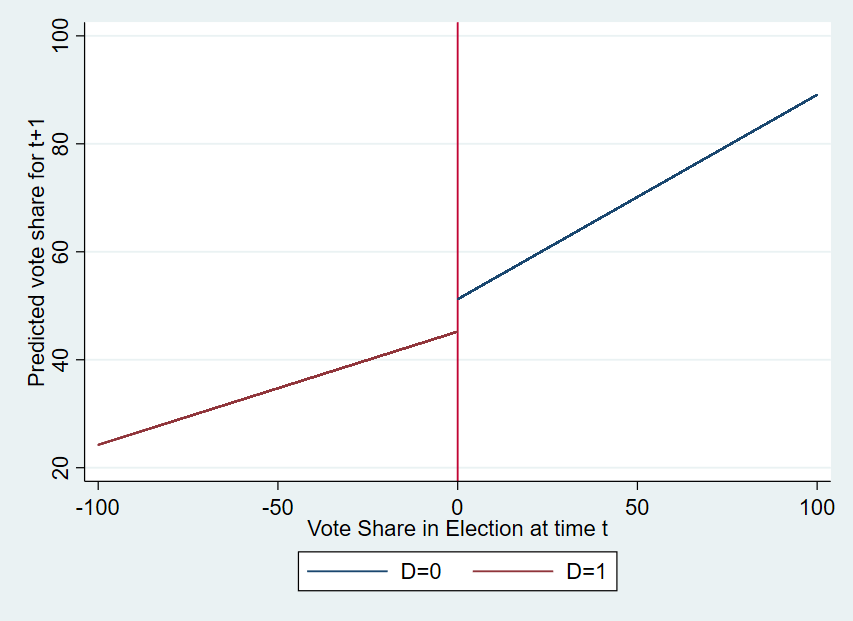
\includegraphics[width=\textwidth]{../Results/7_15_b.png}
            \end{figure}        
        \end{column}

        \begin{column}{0.4\textwidth}
            \begin{align*}
                Y &= \alpha_1 + \alpha_2 X + D(\beta_1 + \beta_2 X) \\
                &=reg~Y ~X~D~XD
            \end{align*}
        \end{column}
    \end{columns}
    


    

\end{frame}
\end{document}